\documentclass[10pt,twocolumntoc]{cekarticle}
\usepackage{amsmath}
\usepackage{amssymb}
\usepackage{array}
\latexhtml{
  \usepackage[american]{varioref}
}{
  \newcommand{\vref}[1]{\ref{#1}}
}

% Aliases for bibliography entries, to compensate for some issues.

\defcitealias{bipm:1998}{BIPM, 1998}
\defcitealias{bipm:2000}{BIPM, 2000}

% Miscellaneous macros.

\newcommand{\D}{\displaystyle}
\newcommand{\tm}{\textsuperscript{\tiny{\texttrademark}}}

%\pagestyle{myheadings}
%\markboth{\textit{SBML Level 2: Working Draft Revision 3}}{\textit{SBML
%    Level 2: Working Draft Revision 3}}

\begin{document}

%=============================================================================
% Title page
%=============================================================================

\title{Parameter Sets: a standard technology for use with SBML}

\author{Andrew Finney, Michael Hucka, Ben Bornstein}

\authoremail{\{afinney,mhucka\}@cds.caltech.edu}

\address{Systems Biology Workbench Development Group\\
  ERATO Kitano Systems Biology Project\\
  Control and Dynamical Systems, MC 107-81\\
  California Institute of Technology, Pasadena, CA 91125, USA\\[3pt]
  \url{http://www.cds.caltech.edu/erato}}

\acknowledge{Principal Investigators: John Doyle and Hiroaki Kitano}

\date{\today{}}

\maketitlepage

%=============================================================================
\section{Introduction}
\label{sec:introduction}
%=============================================================================

This white paper discusses Parameter Sets, a possible new standard interchange format
or technology for use with SBML~\citep{hucka:2001}.  Parameter sets are designed to facilitate the
separation of the initial condition and parameter values of a model from the model structure
itself. In its most basic form a parameter set is
a collection of \emph{key value pairs} where the key refers to an object attribute in an SBML
data source and the value is a new value for the referenced attribute.  A parameter set
can be applied to an existing model: a new model is created in which the attributes of
the original model are substituted according to the key value pairs in the parameter set.
In this document the original document is called the \emph{source} and the new model is
called the \emph{target} model.

\subsection{About this document}

This document outlines a set of requirements for parameter sets in
Section~\ref{sec:requirements}
(similar to a formal "request for proposals") as well as to describe possible implementations
of these requirements in Section~\ref{sec:implementation}.  

The primary purpose
of this document is to present options which the SBML community can discuss and then use
as a framework for constructing a final proposal for a parameter sets standard.  This
document is meant to provoke the discussion of real requirement and practical
implementations rather than providing a definitive statement on either.

\subsection{Brief History of Parameter Sets}

The idea of parameter sets in the context of SBML was first raised as a requirement
publicly by Cliff Schaffer at the BioSPICE MDL meeting in Cambridge, MA in September
2002.  The requirement was discussed on the \emph{sbml-discuss} mailing list.  By
the SBML Forum meeting at ICSB 2002 in December in Stockholm there was a consensus
for some standard development in this area.  Many of the requirements described here
are taken from discussions on the mailing list and at that meeting.  The authors
would like to acknowledge Ben Bornstein's suggestion of using XSLT as an
implementation technology

%=============================================================================
\section{Requirements}
\label{sec:requirements}
%=============================================================================

\subsection{General Motivation}
\label{sec:motivation}

At the start of biochemical network model development many of the parameter values of the 
modelled system are unknown.
As a result a key step of the model development process is finding parameter values which enable 
the model exhibit the same behaviors as the biological system under study. In addition many
researchers argue that one of the key tasks in model development is establishing the robustness 
and fragilities of a given model to specific parameters values. Thus in the majority of cases
during model development the values of parameters and initial conditions are generally more
volatile than the model structure as either human or automated processes explore the parameter 
space of a model.  The result is one or more parameter sets none of which can be described as
definitive.  Modelling tools operate on these parameter sets independently of the model to
which they are applied.

A project may build several models of the same organism for which it has a large set of
experimental data.  The experimental data is stored or made available in the form of a parameter 
set which is applied to the models constructed by the project.  Managing the parameter data in
this way ensures that experimental data can (a) be used consistently across several models and
(b) be updated without requiring model data to be changed.

The following sections describe various features of parameter sets that may (or perhaps not) be
required:

\subsection{Overloading}

The attribute values contained in a parameter set supply values for missing attributes but also
replace existing values in a model that the set is applied to.

The attribute values in a model are typically viewed as more definitive than
those in a parameter set however the values in the parameter set may contain a reasonable set of
alternative values given incomplete experimental results.  A sets of one or more mutations
can be modelled as a set of alternative parameter values.

\subsection{Incomplete}

A parameter set can be incomplete: a parameter set may not necessarily contain values for all
relevant attributes in a given model.

Only a subset of parameter values may be explored during the construction of a model as some
attributes values are more definitive than others e.g. they are the result of accurate
experimental techniques.  In most cases a given mutation only affects
a small subset of model attributes thus a mutation would be best represented using a parameter
set that has value for a subset of attributes.

\subsection{Attributes not in Source Model}

A parameter set may contain values for attributes that are not in the source model, in which
case these values are ignored.

If a parameter set is used as a ``database'' of values taken form experiments that are to be
applied to several models then it is unlikely that all models will use all the attribute values
stored in the parameter set.

\subsection{Cascading}
\label{sec:cascading}
A target model can be described by a sequence of parameters sets combined with a source model.
Each parameter set overloads the attribute values defined by the previous parameter set or
the original model

This enables, for example, a parameter set describing a mutant to be combined with a parameter
set derived by optimization for the same model.

\subsection{Model specificity}
\label{sec:specificity}
A parameter set may or may not be specific to a given source model.  A parameter set should
have an optional field that refers to a specific model.  It is not clear whether the standard
should or can enforce the correct use of this field.  The use of this field enables a target
model to be assembled starting from just a parameter set.  When a parameter set is part of a
cascade this field refers to the previous parameter set in the sequence starting from the
source model.

A parameter set may have attribute values that have been fitted to a specific model in other
cases a parameter set may be a ``database'' of values taken form experiments that are to be
applied to several models.

\subsection{Parameter Sets as Independent Data Stores}
\label{sec:datastore}
Whilst parameter sets primarily are used as transformations on source models, they should support
reading and writing operations on the parameter set.  Ideally these operations should be possible
without reference to a source model.  For example given the identifier for a species it should be
possible to read and the change the species initial concentration in the parameter set without
referring to a model.

There will probably be a tension between this requirement and the requirement for extendability
(see Section~\ref{sec:extendability}) because a generic format may be difficult to parse without
the source model.

\subsection{Extendability}
\label{sec:extendability}
The parameter set form should ideally use a form which ensures that it can be applied to
all current and future forms of SBML.  Such a form is necessarily generic.

Having a generic form will ensure that parameter sets can easily be applied to the potentially
complex forms that could arise in SBML Level 3.

\subsection{Scope of Transformation}

It is not clear what operations a parameter set could apply to a source model to generate a
target model.  Should a parameter set be restricted just to setting alternative attributes
values? For example should a parameter set insert or remove elements?  If we restrict changes
just to overloading attribute values do we need to limit the set of attributes that can be
changed?

For the moment the consensus appears to be that at a minimum parameter values and initial
conditions (species concentration and compartment volumes) can be overloaded by parameter sets.

\subsection{Reference to Expanded Form and Interface Conformance}
\label{sec:implied-structures}

It is possible that a parameter set could refer to objects that are implied by the source
model but that do not exist explicitly in the source model's XML encoding.  A parameter set
may refer to attributes in some expanded form derived from the source model.

For example a
SBML Level 3 source model may contain several instances of a sub-model.  The sub-model may
contain a number of parameters.  A parameter set for this source model may contain attribute
values for the parameters in specific instances of the sub-models even though there are no
explicit structures in the XML for those parameters.

In the use case described above the overloaded parameters are either not part of the declared
interface for the sub-model or the source model assumes default values for the parameters.  The
consensus appears to support the use of parameter sets that ignore or bypass any explicit
sub-model interfaces.

[It is possible that the definition of complex species will make it possible to refer to
reactions and species that are not explicitly listed in a source model.  For example consider a
source model containing a template reaction: a reaction definition, that can be applied to set
of configurations of complex species. A template reaction represents, in SBML Level 2 terms, a set
of reactions.  A parameter set entry could be applied to the rate of a specific reaction instance (or
set of reaction instances) of a template reaction.]

\subsection{Simultaneous Support for Multiple levels}

Given the requirement that a parameter set can be used with more than one model then it should be
possible for a given parameter set to be applied to models encoded in different levels of SBML.

\subsection{Units}

A parameter set can overload an attribute value using different units than those given
in the source model.  The parameter set should use a unit definition from the source model or
provide an alternative unit definition.  The units should address the same physical phenomena as
the target model's unit definition (in most cases this simply means a scale difference).

\subsection{Abstraction}

It is conceivable that a parameter set may wish to derive the values initial conditions and
parameters of a given model from each other i.e. one value is calculated via another.

This capability is not yet available in SBML itself.  It is not clear that parameter sets are
the best place for these math constructs.  For the purposes of this document we assume
that this requirement is best addressed in the context of SBML Level 3.

\subsection{Best Practice}

A best practice document for the use of parameter sets will be required. For exchange between 
software applications target models can be potentially exchanged as a single reference to the last
parameter set in a cascade of parameter set (each parameter set refers the previous set through
to the source model). Alternatively target models could be exchanged with an explicit parameter
set sequence (a set of references).

If model has one definitive set of parameter values then that set
should be contained within the model.  If a model is published in a context where more than one
set of parameters described, in for example text, then those sets should be supplied in parameter
sets as opposed to separate models.  Parameter sets should be used to describe alternative parameter
sets for defining mutations.
%=============================================================================
\section{Implementation}
\label{sec:implementation}
%=============================================================================

\subsection{XSLT}

As parameter sets operate as transforms of source models it is natural to consider the generic XML
transformation technology: the Extensible Stylesheet Language Transformations (XSLT)~\cite{clark:1999}.
This standard is well documented so rather than give an detailed explanation of this technology I
will simply give a simple example.

Consider the following Level 2 model fragment:
\begin{example}
...
<species id="P0" boundaryCondition="false" initialAmount="0" compartment="compartment"/>
<species id="T0" boundaryCondition="false" initialAmount="0" compartment="compartment"/>
<species id="P1" boundaryCondition="false" initialAmount="0" compartment="compartment"/>
<species id="T1" boundaryCondition="false" initialAmount="0" compartment="compartment"/>
<species id="P2" boundaryCondition="false" initialAmount="0" compartment="compartment"/>
<species id="T2" boundaryCondition="false" initialAmount="0" compartment="compartment"/>
<species id="C" boundaryCondition="false" initialAmount="0" compartment="compartment"/>
<species id="Cn" boundaryCondition="false" initialAmount="0" compartment="compartment"/>
...
<reaction id="J23" reversible="false">
<listOfReactants>
  <speciesReference species="Mt" stoichiometry="1" /> 
</listOfReactants>
<listOfProducts>
  <speciesReference species="NN" stoichiometry="1" /> 
</listOfProducts>
<kineticLaw>
<math xmlns="http://www.w3.org/1998/MathML">
  ...
</math>
<listOfParameters>
  <parameter id="kd_24" value="0.01" /> 
  <parameter id="V_24" value="1.2" /> 
  <parameter id="Km_24" value="0.2" /> 
</listOfParameters>
</kineticLaw>
</reaction>
...
\end{example}

If we apply the following XSLT to this model:
\begin{example}
<?xml version="1.0" encoding="UTF-8"?>

<xsl:stylesheet  xmlns:xsl="http://www.w3.org/1999/XSL/Transform" version="1.1"
    xmlns:sbml="http://www.sbml.org/sbml/level2" exclude-result-prefixes="sbml">

<xsl:template match="sbml:species[@id='P0']/@initialAmount">
<xsl:attribute name="initialAmount">5</xsl:attribute>
</xsl:template>

<xsl:template match="sbml:species[@id='C']/@initialAmount">
<xsl:attribute name="initialAmount">10</xsl:attribute>
</xsl:template>

<xsl:template match="@*|node()" >
  <xsl:copy>
    <xsl:apply-templates select="@*|node()"/>
  </xsl:copy>
</xsl:template>
</xsl:stylesheet>
\end{example}

The first two \texttt{template} elements overload the initial concentrations of species
\texttt{P0} and \texttt{C} substituting values of 5 and 10 respectively.  The final
\texttt{template} element simply copies all other structures to the output.

We can cascade this parameter set with the following parameter set:

\begin{example}
<?xml version="1.0" encoding="UTF-8"?>

<xsl:stylesheet  xmlns:xsl="http://www.w3.org/1999/XSL/Transform" version="1.1"
    xmlns:sbml="http://www.sbml.org/sbml/level2" exclude-result-prefixes="sbml">

<xsl:import href="justa.xsl"/>

<xsl:template match="sbml:species[@id='C']/@initialAmount">
<xsl:attribute name="initialAmount">20</xsl:attribute>
</xsl:template>

<xsl:template match="sbml:reaction[@id='J23']//sbml:parameter[@id='V_24']/@value">
<xsl:attribute name="value">1.2</xsl:attribute>
</xsl:template>

</xsl:stylesheet>
\end{example} 

The first \texttt{template} element overloads the previous \texttt{template} element to
set the initial concentration of \texttt{C} to 20.  The second \texttt{template} element 
replaces the value of the \texttt{V\_24} parameter with 1.2.

The \texttt{import} element doesn't implement cascading in exactly the form described in
section~\ref{sec:cascading}.  The cascading overloads the matching of \texttt{template}
elements rather than creating a pipeline of transformations.  The effect is roughly the same
however.

To enable the XSLT to easily parsed independently of a model the form of the XSLT to be used
is restricted.  The last template element is always the recursive copy \texttt{template}
element unless the XSLT imports that element as shown in the examples above.  All other
\texttt{template} elements will simply contain \texttt{attribute} elements.  The value
of the \texttt{template} \texttt{match} attribute will contain the abbreviated XPATH form
shown in the examples.  These XPATH strings can contain only references to SBML \texttt{reaction},
\texttt{parameter}, \texttt{species}, and \texttt{compartment} elements.  Matches to these elements
must be qualified with an equality match to their \texttt{id} attributes.  The last part of the XPATH
string must consist of a match to \texttt{value}, \texttt{initialAmount} or \texttt{volume} attributes.

The disadvantages of XSLT are:
\begin{itemize}

\item can't support transformation of implied structures but only those structures
explicitly in the source model.  This can be only overcome by defining the form of the
implied structures or expanded form.  See section~\ref{sec:implied-structures}.

\item parsing XSLT as a parameter set
independently of a source model is difficult and requires a restricted form of
XSLT to be defined as the parameter set format standard.  

\item one parameter set can't be applied to both Level 1 and Level 2 without duplicating
information (by duplicating templates).

\item no way to optionally apply the XSLT to a specific model
\item cascading will require the careful application of \texttt{import} elements

\end{itemize}

The advantages of using XSLT are:
\begin{itemize}
\item existing well documented and well supported standard
\item very wide scope of transformation
\item will support all future levels of SBML
\item all other requirements of parameter sets are met by XSLT.
\end{itemize}

\subsection{Model Composition}

An alternative approach would be to use the model composition proposal~\citep{finney:2003b}
as an implementation of parameter sets i.e. a proposed form of SBML Level 3.

Although the requirements of model composition do overlap with that
of parameter sets - in both cases an overloading mechanism is needed - there some important differences:

\begin{itemize}
\item The result of model composition is a nested set of model instances
whereas a parameter set simply transforms a model.  
\item Model composition is
always applied to specific submodels whereas parameter sets do not always specify the model that they
are applied to (see section~\ref{sec:specificity}).
\item Model composition can be applied to several submodels where as parameter sets are applied to one model at a time
\end{itemize}
Therefore we describe here a number modifications to the model composition proposal to support its use as parameter sets:

\begin{itemize}
\item The \class{Sbml} type has an optional attribute \attrib{mode} which indicates whether the stream should be interpreted as a parameter set.
\item The stream must contain one and only one \class{Instance} structure which represents the source model.
\item The \class{Instance} type has optional links to specific submodels.
\item Direct links cannot be used (\class{ObjectRef} structures can't be used outside \class{Link} structures).
\item All objects declared in the stream must be linked to structures in the instance.
\item The result of the stream is a transformed version of the model referenced by the instance in which the outer layer of nesting is ignored:
objects inside the instance are at the top level and retain their previous identity.
\end{itemize}

The new form of \class{Sbml} is shown in the UML diagram in figure~\ref{fig:sbml}.

\begin{figure}[h]
  \vspace*{8pt}
  \centering
  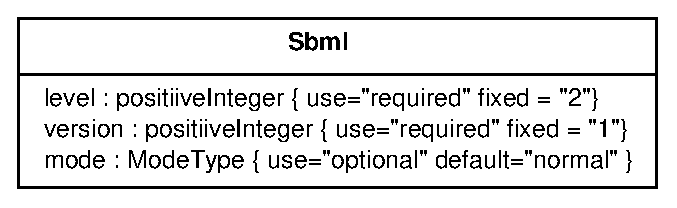
\includegraphics[scale = 0.7]{sbml}
  \caption{The revised \class{Sbml} type}
  \label{fig:sbml}
\end{figure}

The new mode \attrib{mode} can contain one of two values: \emph{normal} or \emph{parameter-set}.
The field defaults to \emph{normal}.  The value \emph{parameter-set} indicates that the stream
should be interpreted as a parameter set.

The new form of \class{Instance} is shown in the UML diagram in figure~\ref{fig:instance}.

\begin{figure}[h]
  \vspace*{8pt}
  \centering
  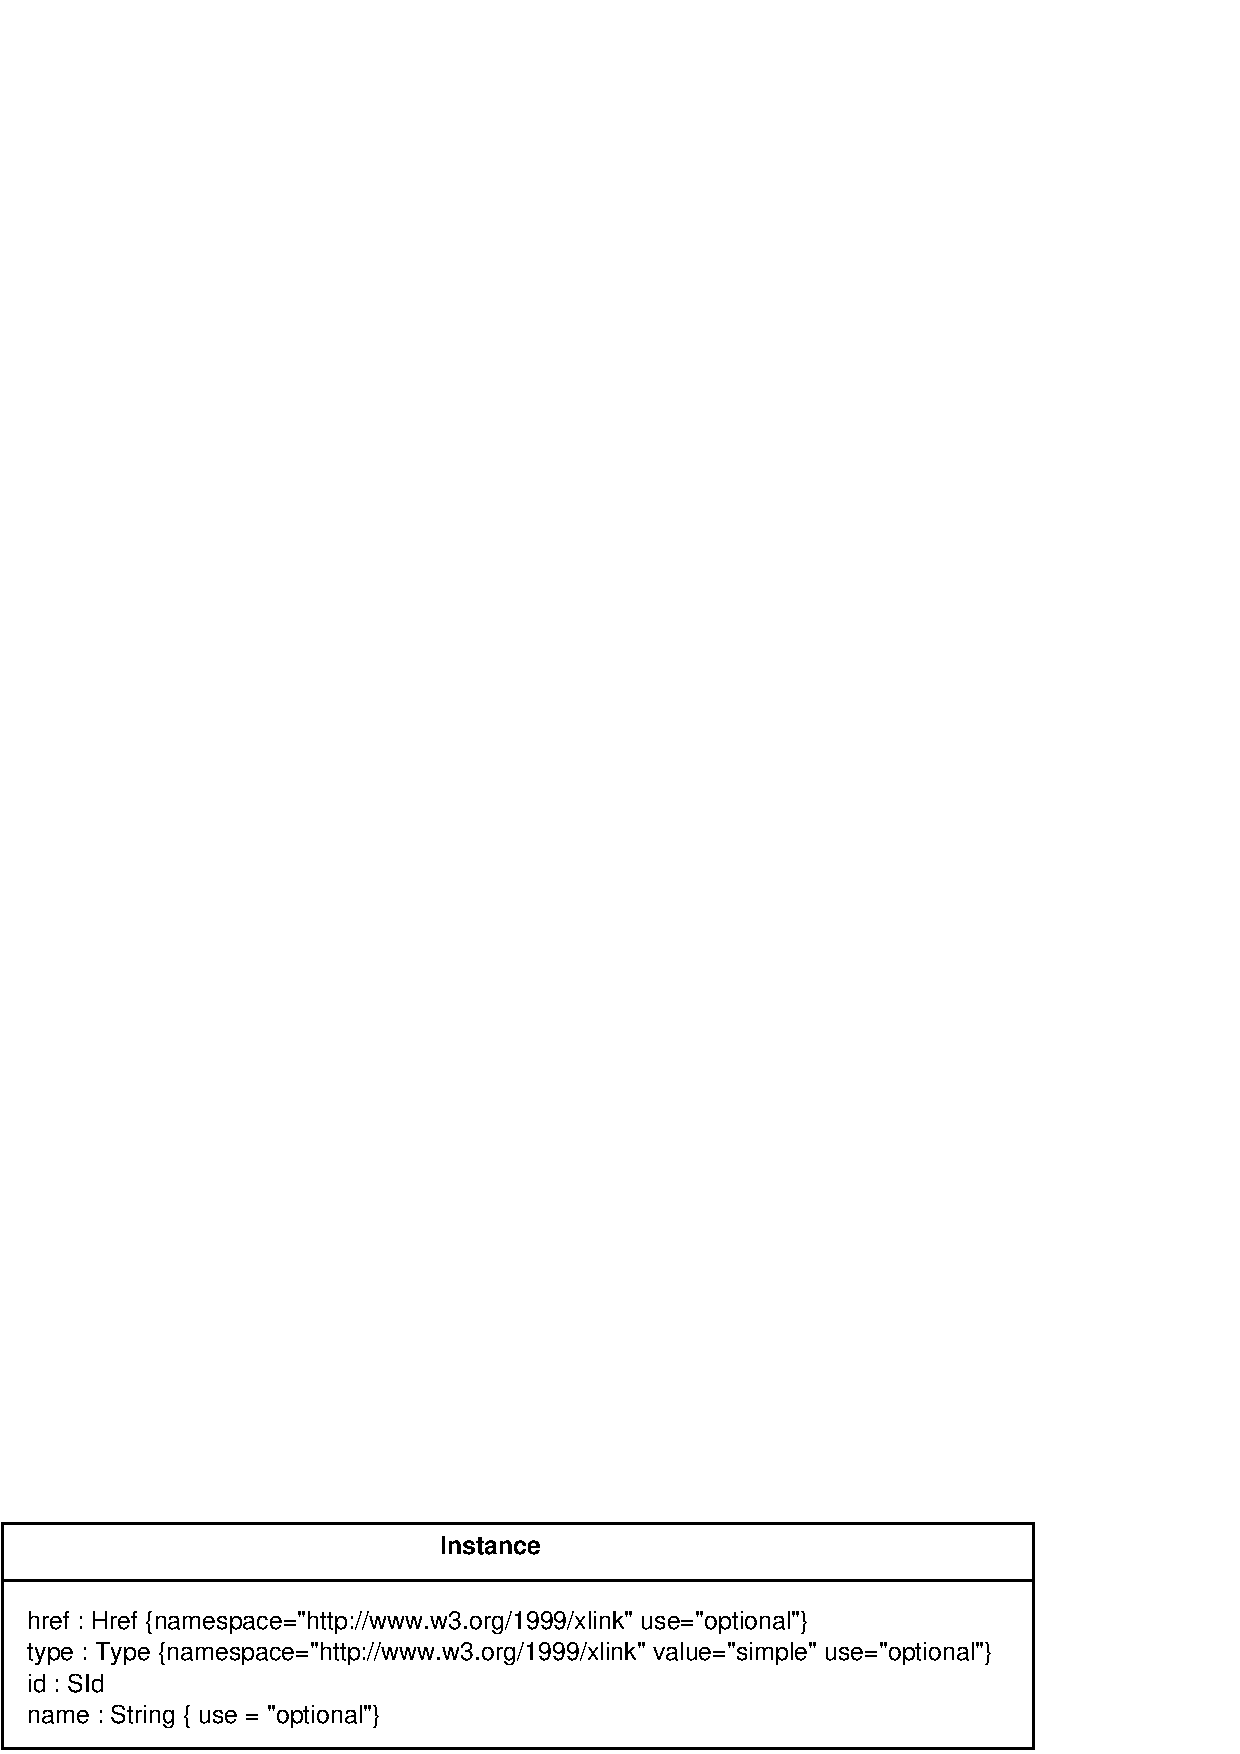
\includegraphics[scale = 0.7]{instance}
  \caption{The revised \class{Instance} type}
  \label{fig:instance}
\end{figure}

In the revised type the XLink attributes are optional.  A \class{Instance} structure which does not
include these attributes is applied to a submodel supplied by the parsing environment.

As an example of this revised form of model composition being used to implement parameter sets
here are the parameter sets corresponding the XSLT transformations given above.
First a parameter set overloading the initial concentrations of species \texttt{P0} and \texttt{C}.
This example uses unlocated species to supply the initial species concentrations.

\begin{example}
<?xml version="1.0"?>
<sbml xmlns="http://www.sbml.org/sbml/level3" version="1" level="3" mode="parameter-set">
    <model id="parameter_set">
        <listOfSpecies>
            <species id="P0" initialAmount=10"/>
            <species id="C" initialAmount="5"/>
        </listOfSpecies>
        <listOfInstances>
            <instance id="source"/>
        </listOfInstances>
        <listOfLinks>
            <link>
                <from object="P0"/>
                <to object="source">
                    <subobject object="P0"/>
                </to>
            </link>
            <link>
                <from object="C"/>
                <to object="source">
                    <subobject object="C"/>
                </to>
            </link>
        </listOfLinks>
    </model>
</sbml>
\end{example}

The following example shows how the previous example cascaded can be overloaded.

\begin{example}
<?xml version="1.0"?>
<sbml xmlns="http://www.sbml.org/sbml/level3" version="1" level="3" mode="parameter-set">
    <model id="cascading_set">
        <listOfSpecies>
            <species id="C" initialAmount="20"/>
        </listOfSpecies>
        <listOfParameters>
            <parameter id="J23__V_24" value="1.2"/>
        </listOfParameters>
        <listOfInstances>
            <instance id="source" xsl:type="simple" xsl:href="justa.xml"/>
        </listOfInstances>
        <listOfLinks>
            <link>
                <from object="C"/>
                <to object="source">
                    <subobject object="C"/>
                </to>
            </link>
            <link>
                <from object="J23__V_24"/>
                <to object="source">
                    <subobject object="J23">
                        <subobject object="V_24"/>
                    </subobject>
                </to>
            </link>
        </listOfLinks>
    </model>
</sbml>
\end{example}

The first \texttt{link} element overloads the previous parameter set to
set the initial concentration of \texttt{C} to 20.  The second \texttt{template} element 
replaces the value of the \texttt{V\_24} parameter with 1.2.

\subsection{Parameter Set specific Format}

This section describes a new non-generic format for parameter sets as a clear alternative
to XSLT and Model Composition.
There seems to be little point in developing another generic form like XSLT.

The scope of the format described here allows the initial values of parameters, species
concentration and compartment volume to be set.  To support modularity the values of these
parameters in sub-models and specific instances of sub-models can be specified.

The UML form of this format is given in Figure~\ref{fig:uml}.

\begin{figure}[h]
  \vspace*{8pt}
  \centering
  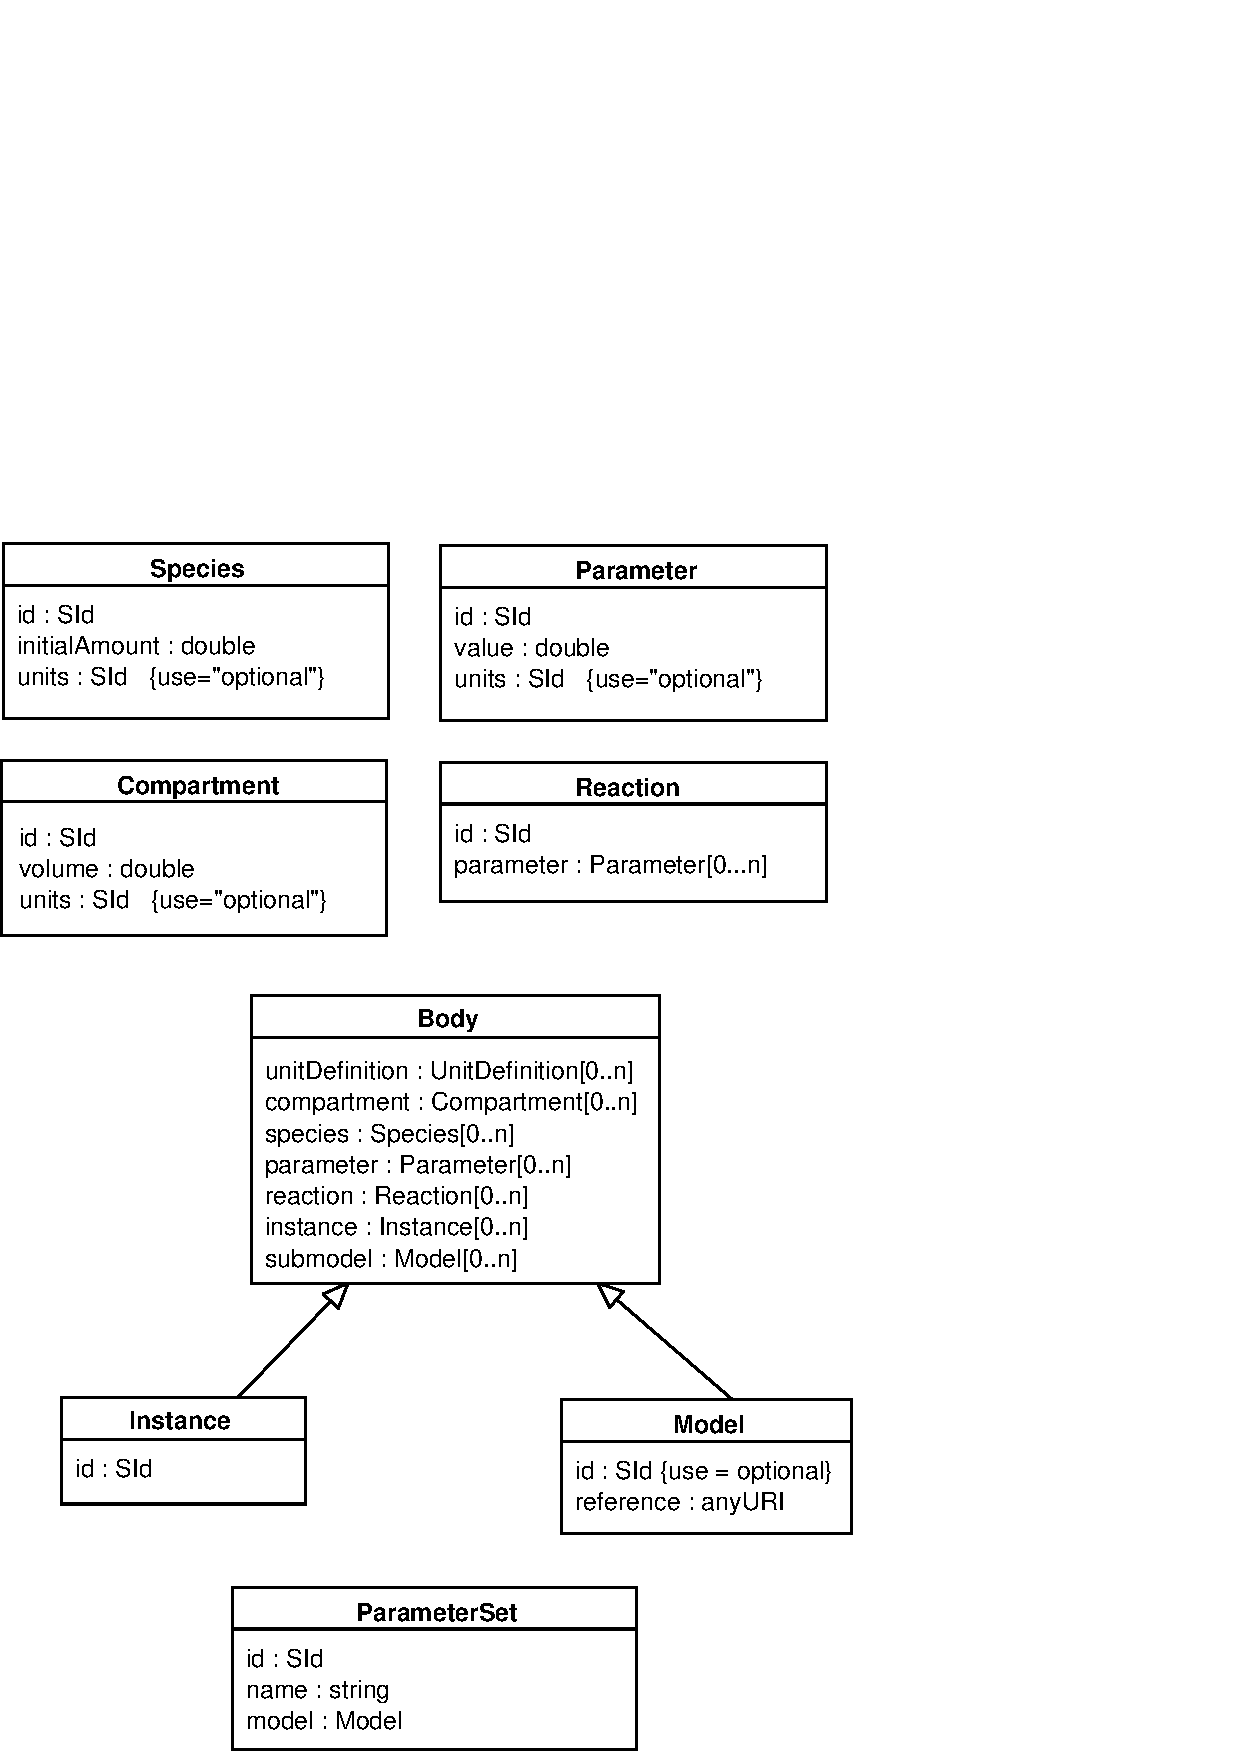
\includegraphics[scale = 0.7]{uml}
  \caption{The UML for a proposed format for parameter sets.  Types without definitions are
  defined in SBML or XML Schema.  \texttt{ParameterSet} is the top level element.}
  \label{fig:uml}
\end{figure}

The top-level element in this format is \texttt{parameterSet} element.  Any element in this\
format, apart from a \texttt{parameterSet} element, refers to an element in SBML with the same
class name and \texttt{id} attribute value.  For example a \texttt{species} element with an
\texttt{id} attribute \texttt{foo} refers to an SBML \texttt{species} element with an
\texttt{id} attribute value \texttt{foo}.  The \texttt{double} type attributes on the
\texttt{species}, \texttt{parameter} and \texttt{compartment} elements
overload the attributes, with same name, on the referenced SBML elements.

The \texttt{reaction}, \texttt{instance} and \texttt{model} elements can enclose other
parameter set elements (to any depth) and define the context in which those enclosed
elements have effect. For example a \texttt{parameter} element enclosed in a
\texttt{reaction} element refers specifically to the SBML \texttt{parameter} element
enclosed in the referenced SBML \texttt{reaction} element.  

The \texttt{parameterSet} element contains a single \texttt{model} element which refers to
the SBML model that the parameter set can be applied to.  This top most \texttt{model}
element has an optional \texttt{id} attribute indicating the model that the parameter set can
be applied to. If this attribute is missing then the parameter set can be applied to an SBML
model with an arbitrary \texttt{id} value. The optional \texttt{reference} attribute contains
the URL of the referenced model or the previous parameter set in a cascade.

As an example here are the parameter sets corresponding the XSLT transformations given above.
First a parameter set overloading the initial concentrations of species \texttt{P0} and \texttt{C}.

\begin{example}
<?xml version="1.0" encoding="UTF-8"?>
<parameterSet xmls="/http://www.sbml.org/parameterSet">
  <model>
    <listOfSpecies>
      <species id="P0" initialAmount="5"/>
      <species id="C" initialAmount="10"/>
    </listOfSpecies>
  </model>
</parameterSet>
\end{example}

Secondly a parameter set, overloading the previous set, setting the initial concentration of species
\texttt{C} and the value of parameter \texttt{V\_24} of reaction \texttt{J23}.

\begin{example}
<?xml version="1.0" encoding="UTF-8"?>
<parameterSet xmls="/http://www.sbml.org/parameterSet">
  <model reference="justa.xml">
    <listOfSpecies>
      <species id="C" initialAmount="20"/>
    </listOfSpecies>
    <listOfReactions>
      <reaction id="J23">
        <listOfParameters>
          <parameter id="V_24" value="1.2"/>
        </listOfParameters>
      </reaction>
    </listOfReactions>
  </model>
</parameterSet>
\end{example}

The \texttt{model} element, as well as containing lists of \texttt{species}, \texttt{parameter}
and \texttt{compartment} elements, contains lists of \texttt{model} and \texttt{instance}
elements to support SBML Level 3 model composition.  Following the pattern outlined above
\texttt{model} elements contained inside other \texttt{model} elements refer to SBML sub-models
and must have an \texttt{id} attribute value. \texttt{instance} elements follow a similar pattern
however the elements enclosed inside \texttt{instance} elements refer to SBML elements in the 
sub-model that the SBML \texttt{instance} is an instance of.  These sub-elements only apply to
the specific instance of the sub-model i.e. the structures ``implied'' by the SBML
\texttt{instance} element.  Whereas the elements enclosed inside \texttt{model} elements refer to
actual SBML elements within the referenced SBML \texttt{model} element those inside
\texttt{instance} elements do not.  At a given hierarchical level the values enclosed in
\texttt{instance} elements overload those enclosed in a \texttt{model} element.

The values of \texttt{units} attributes should be either the \texttt{id} of a
\texttt{unitDefinition} in either the enclosing \texttt{model} element or referenced
SBML \texttt{model} element or a built-in unit such as \texttt{time}, \texttt{volume} or
\texttt{substance}.  The units simply define the units of the double value on the given
element  The unit definition elements must not overload the \texttt{time}, \texttt{volume}
and \texttt{substance} built-ins.

The format described in this section addresses the majority of requirements outlined in
section~\ref{sec:requirements} it is not a generic format and thus cannot be immediately
be used to define a wider range of transformations or be applied to later SBML Levels
without defining more elements for the format.

%\newpage
%\section{Appendix}
%\setcounter{secnumdepth}{2}
%\appendix

\clearpage

%=============================================================================
% References
%=============================================================================

\bibliographystyle{apalike}
\bibliography{strings,a,b,c,d,e,f,g,h,i,j,k,l,m,n,o,p,q,r,s,t,u,v,w,x,y,z}

%=============================================================================
% The end.
%=============================================================================

\end{document}
